\documentclass[]{scrreprt}
\usepackage{amsmath,amsfonts,graphicx}
\usepackage{multirow}
\usepackage{pslatex}
\usepackage{tabularx}
\usepackage{comment}
\usepackage{xspace}
\usepackage{array}

\usepackage{hyperref}

\usepackage{caption}
\DeclareCaptionFont{white}{\color{white}}
\DeclareCaptionFormat{listing}{\colorbox{gray}{\parbox{\textwidth}{#1#2#3}}}

\graphicspath{
{figures/}
}

\newcommand{\uo}{\mbox{UO\textsubscript{2}}\xspace}

\setcounter{secnumdepth}{3}


\begin{document}


\title{Adsorption and Desorption}
\author{Andy Wilkins \\
CSIRO}
\maketitle

\tableofcontents

%%%
\chapter{Theory}
%%%

The reactive transport module of MOOSE\footnote{L Guo, H Huang, DR
  Gaston, CJ Permann, D Andrs, GD Redden, C Lu, DT Fox, Y Fujita, ``A
  parallel, fully coupled, fully implicit solution to reactive
  transport in porous media using the preconditioned Jacobian-Free
  Newton-Krylov Method'' Advances in Water Resources 53 (2013)
  101--108} solves quite general advection-dispersion-reaction
equations.  Such equations are found in porous media, for example.  The
adsorption/desorption kernels described herein are a small addition to
such scenarios.  They can also be used to describe adsorption and
desorption in systems governed by the multi-phase Richards' equation.

The adsorption/desorption equation is
\begin{equation}
\dot{C} = \left\{
\begin{array}{ll}
-(C - C_{\mathrm{e}})/\tau_{d} & \ \ \ \mbox{for } \ \ C\geq C_{\mathrm{e}} \\
-(C - C_{\mathrm{e}})/\tau_{a} & \ \ \ \mbox{for } \ \ C < C_{\mathrm{e}} 
\ .
\end{array}
\right.
\label{eqn.adde}
\end{equation}
In this equation:
\begin{itemize}
\item $C = C(x,t)$ is the adsorbed concentration of a fluid (mass/volume,
  usually kg.m$^{-3}$).  In the porous-media setting, $C$ is the
  concentration of the fluid within the matrix of the
  porous medium, for example, the concentration of methane adsorbed
  into the coal matrix.   Note the units: experiments often quote
  concentration as mass-of-fluid-at-standard-temperature-and-pressure
  divided by mass-of-matrix.  To convert such an experimental value to
  $C$, the experimental value must be multiplied by the density of the
  fluid at standard temperature and pressure.
\item $\tau_{d}$ is the time-constant for desorption.
\item $\tau_{a}$ is the time-constant for adsorption.
\item $C_{\mathrm{e}}$ is the equilibrium concentration, described
  more fully below
\end{itemize}
The governing equation is therefore free of spatial derivatives, and
is just a Newton-cooling equation.

In many cases the fluid is desorbed from the matrix into the porespace
(and adsorbed from the porespace back to the matrix), and there is
another equation governing the mass of the fluid in the porespace:
\begin{equation}
\dot{\rho} = \frac{1}{\tau}(C - C_{\mathrm{e}})
+ \ldots\ .
\label{porespace.eqn}
\end{equation}
Here $\rho$ is the mass density of the fluid in the porespace (which
is usually the product of porosity, density and saturation of the
fluid).  The $(C-C_{\mathrm{e}})/\tau$ term is the rate of desorption
(with $\tau=\tau_{d}$) or adsorption (with $\tau=\tau_{a}$)
from the matrix to the porespace.  The final ``$\ldots$'' represent
other physics, such as advection or dispersion which are unimportant
here.

Finally, $C_{\mathrm{e}}$ must be defined, and there are many
different possible forms.  So far I have only coded the Langmuir
version, which is defined by
\begin{equation}
C_{\mathrm{e}} = \frac{\rho_{L}P}{P+P_{L}} \ .
\label{langmuir.ce}
\end{equation}
In this equation $\rho_{L}$ is the ``Langmuir density'' (measured in
mass/volume, usually kg.m$^{-3}$).  Usually the Langmuir {\em volume}
is used, which is the volume of adsorbed gas at standard temperature
and pressure, divided by the volume of the matrix.  This is
inconvenient in MOOSE as everything else is measured in mass/volume.
Therefore, the usual Langmuir volume must be multiplied by the density
of gas at standard temperature and pressure to yield the ``Langmuir
density'':
\begin{equation}
\rho_{L} = V_{L}\times \rho_{\mathrm{stp}} \ .
\end{equation}
$P_{L}$ is the ``Langmuir pressure'' (with
the same units as $P$).  $P$ is the (partial) pressure of the fluid in
the porespace that appears in Eqn~(\ref{porespace.eqn}).



\chapter{MOOSE implementation}

The RHSs of Eqn~(\ref{eqn.adde}) and Eqn~(\ref{porespace.eqn}) (without
the $\ldots$ terms) have been coded as two Kernels.  The reason for
having two, rather than one, is to make the Jacobian contributions
simple.

The Langmuir equilibrium concentration, Eqn~(\ref{langmuir.ce}), has
been coded into a Material class, which stores $\rho_{L}$ and $P_{L}$,
and calculates $C_{\mathrm{e}}$ as well as its derivative with respect
to $P$.  By doing this, rather than getting the Kernels to calculate
$C_{\mathrm{e}}$, I hope future developers will be able to more
easily code different forms for $C_{\mathrm{e}}$.


\chapter{Tests}

It is sufficient to test the following system of equations
\begin{eqnarray}
\dot{C} & = & -(C-C_{\mathrm{e}})/\tau \ , \nonumber \\
\dot{P} & = & (C-C_{\mathrm{e}})/\tau \ , \nonumber \\
C_{\mathrm{e}} & = & \frac{\rho_{L}P}{P_{L}+P} \ .
\label{test.eqns}
\end{eqnarray}
These equations are not supposed to be physically meaningful (for
instance, $P_{L}$ has dimensions mass/volume), but they have simple
solutions.  I have used $\tau = \tau_{d} = \tau_{a}$.

\section{A test of the Jacobian}

The Jacobians of the two Kernels both involve diagonal terms
(derivatives wrt the variable) and off-diagonal terms (derivatives wrt
the other variable).  The automatic test suite uses PETSc's {\tt
  snes\_type=test} (a finite-difference) to test that these Jacobian
entries are correct.

\section{A test of the dynamics}

A single-element model is initialised with $C=1=P$, and $\tau=1.1$,
$\rho_{L}=0.88$ and $P_{L}=1.23$.  The simulation is run to $t=2$, and compared
with an Excel solution of Eqns~(\ref{test.eqns}).  Good agreement is
shown in Figure~\ref{langmuir_test.fig}.  This test is part of the
automatic test suite that is run every time the MOOSE core code is
updated.


\begin{figure}[htb]
\centering
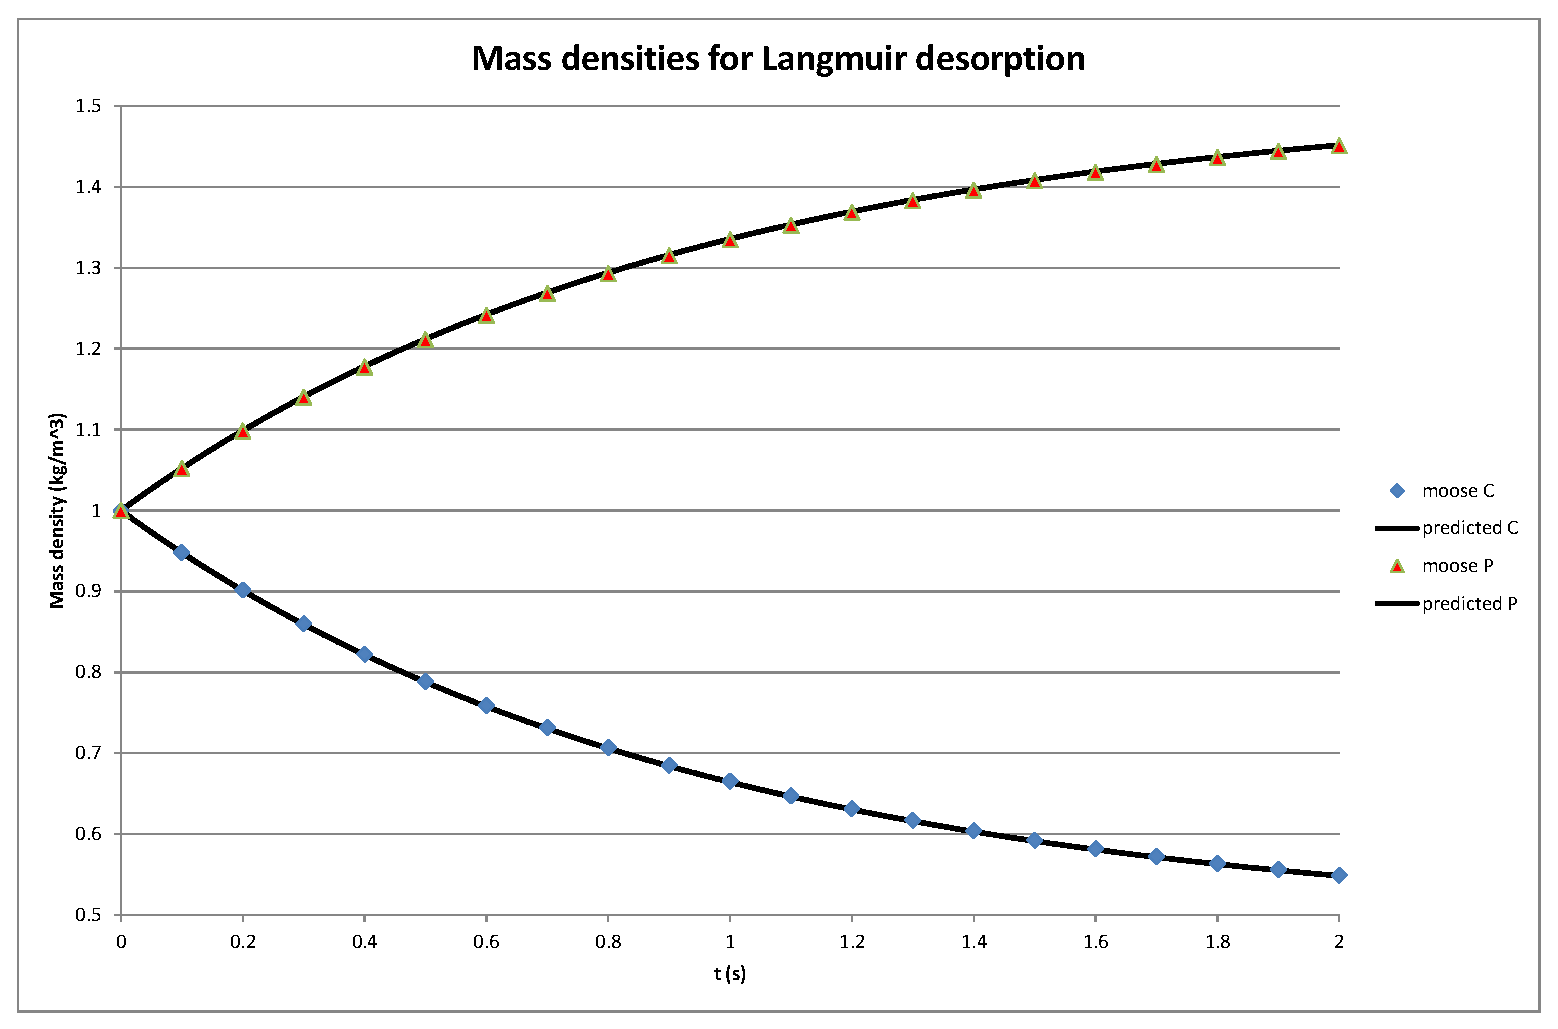
\includegraphics[width=13cm]{langmuir_test.eps}
\caption{Comparison of the MOOSE solution (dots) to Eqn~(\ref{test.eqns}) and
  an Excel solution (lines) demonstrating that MOOSE's implementation of the
  equations is correct.}
\label{langmuir_test.fig}
\end{figure}

\end{document}

